
\chapter{オブジェクト指向入門}

プログラミングは今まで見てきた手続きを関数としてまとめながら記述する方法で作成されています。

プログラムの規模が大きくなるともっと効率よく書く方法が考えられるようになりました。

この方法の一つがオブジェクト指向プログラミングと言われています。オブジェクト指向プログラミングではプログラムコードの
再利用を効率よく行うことできることがメリットです。

この中で重要なキーワードがクラスといわれる考え方で扱うデータと処理(メソッド)を一体化した仕組みを指します。

\section{クラス入門}
\subsection{クラスとは?}

クラスとはデータとデータを処理すべき手続きをひとまとめにして、型として定義したものです。
型は中身の無いものなので、たい焼きの型を思い出していただければと思います。たい焼きの型に小麦粉やクリームなどの材料を入れ加熱調理することで
たい焼きになりますが、このことをインスタンス化(実体化)と言います。

ここでは概略のみの説明となりますので、厳密な定義は各解説書やWebを確認してください。

まずは簡単に学生の名前と1科目の点数と成績を管理するためのクラスを作りたいと思います。


そのためにはクラスの書き方から見ていきましょう。

一番簡単なクラスの定義は次の通りです。一般的にクラス名は英大文字から書くことが多いです。
\begin{verbatim}
class クラス名:
    pass
\end{verbatim}

本来ブロックには1行以上プログラムを記述する必要がありますが、passという何もしないというプログラムコードを
書くことでなにもしないブロックを記述することができます。

\subsection{実体(インスタンス)}
クラスをプログラムから利用するためには変数にクラス定義された型から実体を作る必要がありますので、そのやり方を見ていきましょう。

{\gt 凡例class-1}
なにも機能を持たないクラスの定義を利用したデータの管理を確認します。

変数aもbもそれぞれPersonクラスの実体ですが、別のデータを保管管理することになることを確認しましょう。

それぞれの実体に持たせることができる変数は任意のものを定義することができます。


クラス定義はclassの後にクラス名を書きますが、クラス名の頭文字は大文字にする慣例があります。
{\gt 凡例class1-1.py}
\begin{listing}{1}
#クラス定義
class Person:
    pass #なんの命令もない空クラス(型)
    
#実体の作成 1つ目 変数a、二つ目 変数b
a = Person()
b = Person()
#1つ目の実体のxという変数に10を代入
a.x = 10
#2つ目の実体のxという変数に20を代入
b.x = 20
#1つ目aと二つ目bの実体のxという変数を出力 
print("a.x = ", a.x)
print("b.x = ", b.x)
\end{listing}
実行結果
\begin{listing}{1}
a.x =  10
b.x =  20
\end{listing}


{\gt Point}
何度か実体という言葉がでてきますが、凡例class-1では6行目と7行目でそれぞれ別のものが作られていると考えると
自然かと思います。なにかしら得体のしれないデータを格納できる変数aとbをオブジェクト指向ではインスタンス(実体)と
いうことを覚えておきましょう。

\newpage
\subsection{クラス変数}
凡例class-1では実体1と実体2でそれぞれ別のデータを扱うことがわかりましたが、実体間で共通のデータを扱う方法を考えます。
(厳密には異なりますが、グローバル変数のようなもの)
{\gt 凡例class-2}
クラス変数と言って一つのクラスでは値として一つだけの変数を定義することができます。

変数aもbもそれぞれPersonクラスの実体ですが、クラス変数では共通のデータを管理することになることを確認しましょう。

それぞれの実体に持たせることができる変数は任意のものを定義することができます。

{\gt 凡例class1-2.py}
\begin{listing}{1}
class Person:
    pass

a = Person()
b = Person()
#クラス名の後に変数を記述するとクラス変数となる。
Person.x = 10
#また実体の__class__を利用するとクラス変数となる。
b.__class__.x = 20
#凡例class-1と同じ書き方ですが、それぞれクラス変数と解釈されると
#実体1と実体2で共通の値を参照していることがわかります。
print("a.x = ", a.x)
print("b.x = ", b.x)
\end{listing}
実行結果
\begin{listing}{1}
a.x =  20
b.x =  20
\end{listing}






\subsection{メソッド(オブジェクト内の処理)}
ここまでで説明したデータを持たせることは見ることができましたが、処理(手続き)を持たせたるとはどういうことか見てみたいと思います。

クラス内の処理はメソッド(クラス内の関数の呼び方)といい実体ごとのデータを処理することができます。
\newpage
{\gt 凡例class-3}
ここでは数学(Mathematics)の点数のデータを処理し合格"good"か不合格"bad"を判定する手続きをクラスに記述します。

ここでメソッドset\_mはStudentクラスのブロック中に書かれます。
set\_mの第一引数は自分自身の実体となりますので、実体ごとに管理するデータはselfに「.」をつけることで設定・参照することができます。
{\gt 凡例class1-3.py}
\begin{listing}{1}
class Student: 
    #数学の点数を管理する処理
    def set_m(self,m):
        #第二引数は17行目以降のset_mの引数となり
        #実体のデータmとして管理・操作できるように保存
        self.m = m
        if m >= 50:
            #合否を実体のデータgradingとして設定
            self.grading = "good"
        else:
            self.grading = "bad"

a = Student()
b = Student()
c = Student()
#Studentの中身を知らなくてもset_mが何をするのか知っていればOK
a.set_m(75)
b.set_m(48)
c.set_m(95)
print("a ", a.m ,a.grading)
print("b ", b.m ,b.grading)
print("c ", c.m ,c.grading)
\end{listing}
実行結果
\begin{listing}{1}
a  75 good
b  48 bad
c  95 good
\end{listing}




クラスを利用するとそのクラスの中身を知らなくてもどのような結果を得られるのかということを知っているだけで利用することが可能になります。
{\gt Point}
多くのプログラミングではクラスの形(定義)とそのクラスを利用する方法が一緒に書かれているため、クラスとして書かれたプログラムの内容も
理解しておく必要があると思われがちですが、いままで見てきた配列(リスト)のように.appendやpopなど使い方だけ知っていれば
良いと考えておいてください。


\subsection{クラスの継承}
オブジェクト指向ではクラスの継承というコードの再利用のための仕組みがあります。

ここでは簡単に継承の形式を確認してみましょう。

オブジェクト指向ではベースとなる基盤機能をもっているクラスをスーパークラス、基盤の機能を利用するクラスを
サブクラスといいます。
\begin{center}
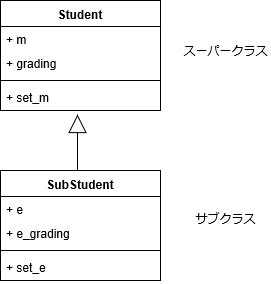
\includegraphics[width=5cm]{images/ClassExtends.png}
\end{center}

サブクラスではスーパークラスの機能を利用することができますので、Studentクラスで定義されているset\_mメソッドやgradingといったデータは
SubStudentクラスで定義していなくても利用できます。
\newpage
{\gt 凡例class-4}
凡例class-3のStudentは(Mathematics)クラスはそのままに(English)の点数のデータを処理し合格"good"か不合格"bad"を判定する
処理set\_eをサブクラスSubStudentに記述します。

{\gt 凡例class1-4.py}
\begin{listing}{1}
class Student: 
    def set_m(self,m):
        self.m = m
        if m >= 50:
            self.grading = "good"
        else:
            self.grading = "bad"
#クラス宣言の括弧の中に利用したい機能のスーパークラスを記載します。
class SubStudent(Student): 
    def set_e(self,e):
        self.e = e
        if e >= 50:
            #合否を実体のデータe_gradingとして設定
            self.e_grading = "good"
        else:
            self.e_grading = "bad"
a = SubStudent()
a.set_m(80)
a.set_e(30)
print("a Mathematics", a.m ,a.grading)
print("a English", a.e ,a.e_grading)
\end{listing}
実行結果
\begin{listing}{1}
a  Mathematics 80 good
a  English 30 bad
\end{listing}





